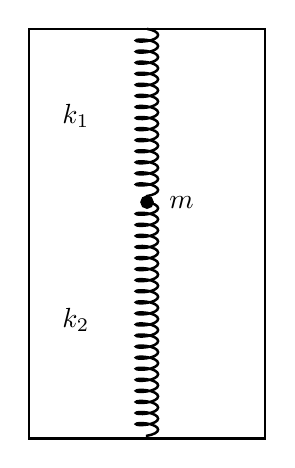
\begin{tikzpicture}[line width=0.9pt]
  % bounding box
  \draw (0,0) rectangle (3,5.2);
  % upper spring k1
  \draw[decorate,decoration={coil,aspect=0.3,segment length=4pt,amplitude=4pt}] (1.5,5.2) -- (1.5,3.0);
  \node[left] at (0.9,4.1) {$k_1$};
  % mass m (dot at junction)
  \filldraw (1.5,3.0) circle (2pt);
  \node[right] at (1.65,3.0) {$m$};
  % lower spring k2
  \draw[decorate,decoration={coil,aspect=0.3,segment length=4pt,amplitude=4pt}] (1.5,3.0) -- (1.5,0);
  \node[left] at (0.9,1.5) {$k_2$};
\end{tikzpicture}
